%4619055 課題3 論理回路
\documentclass[12pt]{jarticle}
\usepackage{TUSIreport}
\usepackage{otf}
\usepackage{graphicx}
\usepackage{amsmath}
\usepackage{amssymb}
\usepackage{hhline}
\usepackage{fancybox,ascmac}
\usepackage{url}
%%%%%%%%%%%%%%%%%%
\begin{document}
%%%%%%%%%%%%%%%%%%%%%%%%%%%%%%%%%%%%%%%%%%%%%%%%%%%%%%%%
% 表紙を出力する場合は,\提出者と\共同実験者をいれる
% \提出者{科目名}{課題名}{提出年}{提出月}{提出日}{学籍番号}{氏名}
% \共同実験者{一人目}{二人目}{..}{..}{..}{..}{..}{八人目}
%%%%%%%%%%%%%%%%%%%%%%%%%%%%%%%%%%%%%%%%%%%%%%%%%%%%%%%
\提出者{情報工学実験1}{課題3 論理回路}
{2020}{6}{15}{4619055}{辰川力駆}

\共同実験者{}{}{}{}{}{}{}{}
\追加実験者{}{}
\表紙出力

\section{実験の目的}
ディジタル回路の設計・解析に必要な基本となるゲート素子(AND、OR、NOT、NAND、NOR、EX-OR)
の基礎的動作原理を理解し、その応用について考察する。

\section{実験概要}
本実験は論理回路実習装置ITF-02を用いて行う。
この装置の使用に当たっては次の注意を守る。
\begin{itemize}
    \item パネル面での結線は必ず電源スイッチをオフにしておく。
    \item リードチップの抜き差しはプラグの部分を持って行う。リード線を持って抜き差しすると断線の原因になる。
    \item パネル面での結線を行う場合には、リードチップがからまないようにその結線に合ったリードチップを使用する。
\end{itemize}
実験は以下に示す順序で行うこと。
\begin{itemize}
    \item[(1)] 論理積(AND)回路
    \item[(2)] 論理和(OR)回路
    \item[(3)] 否定(NOT)回路
    \item[(4)] 論理積の否定(NAND)回路
    \item[(5)] 論理和の否定(NOR)回路
    \item[(6)] ド・モルガンの定理の証明
    \item[(7)] 排他的論理和(EX-OR)回路
    \item[(8)] 加算器(ADDER)の実習
    \item[(9)] デコーダの実習
    \item[(10)] R-Sフリップ・フロップ
    \item[(11)] J-Kフリップ・フロップ
\end{itemize}
\clearpage

\section{実験}
\subsection{操作手順}

本器ITF-02の基本的な操作手順は、次の通りとする。
\begin{itemize}
    \item[1.] 電源スイッチをOFFにする。
    \item[2.] 各実習項目における結線を行う。
    \item[3.] 電源スイッチをONにする。
    \item[4.] 各実習項目における実習を行う。
    \item[5.] 実習が終了したら電源スイッチをOFFにして、結線を解く。
\end{itemize}

<注意>

結線を行ったり、結線を解いたりするときは、原則として電源スイッチをOFFにしておくこと。
ただし、実習を行っている途中で結線を変えたり、結線を増やしたりするときは、
その都度電源スイッチをOFFにする必要はない。
その場合には、出力信号をアースに短絡したり、出力端子と出力端子を接続したりしないよう注意すること。
結線を途中で変えるときは、信号出力端子に差し込んであるリードチップを抜き、
次に信号入力端子に差し込んであるリードチップを抜く。
また、結線を追加するときは、リードチップを信号入力端子に差し込み、次に信号出力端子に差し込む。

\subsection{組み合わせ回路の実習}
組み合わせ回路は、出力が入力だけに関係する論理回路で、基本になる素子として、
論理積(AND)、論理和(OR)、否定(NOT)、論理積の否定(NAND)、論理和の否定(NOR)などがあり、
その応用として排他的論理和(Exclusive-OR)、半加算器(Half-ADDER)、
全加算器(Full-ADDER)、エンコーダ、デコーダなどがある。

\subsubsection*{(1) 論理積(AND)回路}
\begin{itemize}
    \item 目的

          $Y=A\cdot B$ を理解する。

    \item 理論

          論理積は、$Y=A\cdot B$で表現され、
          入力$A$と$B$がいずれも``1"のときのみ、
          出力$Y$が``1"、他の条件ではすべて``0''となるもので、
          この式を満足する論理回路をAND回路という。

          \clearpage

          \begin{table}[h]
              \caption{ANDの真理値表}
              \begin{center}
                  \begin{tabular}{|c|c|c|}
                      \hline
                      A & B & Y \\
                      \hline
                      0 & 0 & 0 \\
                      \hline
                      0 & 1 & 0 \\
                      \hline
                      1 & 0 & 0 \\
                      \hline
                      1 & 1 & 1 \\
                      \hline
                  \end{tabular}
              \end{center}
              \label{table1}
          \end{table}

    \item 実習

          パネル上のAND回路素子を使用し、
          $Y=A\cdot B$の真理値表\ref{table1}を表示器で表示して
          確認することにより行う。

          $A$、$B$の入力レベルは、設定スイッチにより設定する。
\end{itemize}

\subsubsection*{(2) 論理和(OR)回路}
\begin{itemize}
    \item 目的

          $Y = A + B$を理解する。

    \item 理論

          論理和は、$Y= A + B$で表現され、
          入力$A$と$B$がいずれも``0''のときのみ、
          出力$Y$が``0''、他の条件ではすべて``1''となるもので、
          この式を満足する論理回路をOR回路という。

          \begin{table}[h]
              \caption{ORの真理値表}
              \begin{center}
                  \begin{tabular}{|c|c|c|}
                      \hline
                      A & B & Y \\
                      \hline
                      0 & 0 & 0 \\
                      \hline
                      0 & 1 & 1 \\
                      \hline
                      1 & 0 & 1 \\
                      \hline
                      1 & 1 & 1 \\
                      \hline
                  \end{tabular}
              \end{center}
              \label{table2}
          \end{table}

    \item 実習

          パネル上のOR回路素子を使用し、
          $Y = A + B$の真理値表\ref{table2}を表示器で表示して
          確認することにより行う。

          $A$、$B$の入力レベルは、設定スイッチにより設定する。
\end{itemize}

\subsubsection*{(3) 否定(NOT)回路}
\begin{itemize}
    \item 目的

          $Y = \overline{A}$を理解する。

    \item 理論

          否定回路は、インバータとも言われ、$Y = \overline{A}$で表現される。
          入力と出力の関係は常に正反対になり、
          この式を満足する論理回路を否定回路という。

          \begin{table}[h]
              \caption{NOTの真理値表}
              \begin{center}
                  \begin{tabular}{|c|c|}
                      \hline
                      A & Y \\
                      \hline
                      0 & 1 \\
                      \hline
                      1 & 0 \\
                      \hline
                  \end{tabular}
              \end{center}
              \label{table3}
          \end{table}

    \item 実習

          パネル上のNOT回路素子を使用し、
          入力Aに対し出力$Y = \overline{A}$の真理値表\ref{table3}を表示器で表示して
          確認することにより行う。

          $A$、$B$の入力レベルは、設定スイッチにより設定する。
\end{itemize}

\subsubsection*{(4) 論理積の否定(NAND)回路}
\begin{itemize}
    \item 目的

          $Y = \overline{A \cdot B}$ を理解する。

    \item 理論

          論理積の否定は、$Y = \overline{A \cdot B}$で表現され、
          入力$A$と$B$がいずれも``1''のときのみ、出力$Y$が ``0''、
          他の条件ではすべて``1''となるもので、
          この式を満足する論理回路をNAND回路という。

          \begin{table}[h]
              \caption{NANDの真理値表}
              \begin{center}
                  \begin{tabular}{|c|c|c|}
                      \hline
                      A & B & Y \\
                      \hline
                      0 & 0 & 1 \\
                      \hline
                      0 & 1 & 1 \\
                      \hline
                      1 & 0 & 1 \\
                      \hline
                      1 & 1 & 0 \\
                      \hline
                  \end{tabular}
              \end{center}
              \label{table4}
          \end{table}

    \item 実習

          パネル上のNAND回路素子を使用し、
          $Y = \overline{A \cdot B}$の
          真理値表\ref{table4}を表示器で表示して
          確認することにより行う。

          $A$、$B$の入力レベルは、設定スイッチにより設定する。
\end{itemize}

\clearpage

\subsubsection*{(5) 論理和の否定(NOR)回路}
\begin{itemize}
    \item 目的

          $Y = \overline{A + B}$を理解する。
    \item 理論

          論理和の否定は、$Y = \overline{A + B}$で表現され、
          入力$A$と$B$がいずれも``0''のときのみ、
          出力$Y$が``1''、他の条件ではすべて``0''となるもので、
          この式を満足する論理回路をNOR回路という。

          \begin{table}[h]
              \caption{NORの真理値表}
              \begin{center}
                  \begin{tabular}{|c|c|c|}
                      \hline
                      A & B & Y \\
                      \hline
                      0 & 0 & 1 \\
                      \hline
                      0 & 1 & 0 \\
                      \hline
                      1 & 0 & 0 \\
                      \hline
                      1 & 1 & 0 \\
                      \hline
                  \end{tabular}
              \end{center}
              \label{table5}
          \end{table}
    \item 実習

          パネル上のNOR回路素子を使用し、
          $Y = \overline{A + B}$の
          真理値表\ref{table5}を表示器で表示して
          確認することにより行う。

          $A$、$B$の入力レベルは、設定スイッチにより設定する。
\end{itemize}

\subsubsection*{(6) ド・モルガンの定理の証明}
\begin{itemize}
    \item 目的

          ド・モルガンの定理証明として、

          $ \overline{A \cdot B} = \overline{A} + \overline{B} $

          $\overline{A + B} = \overline{A} \cdot \overline{B}$

          の式に、実際の値を入れて行う。

    \item 理論

          ド・モルガンの定理は、式(\ref{eq1})、 および式(\ref{eq2})で表示される。
          \begin{eqnarray}
              \overline{A \cdot B} = \overline{A} + \overline{B} \label{eq1} \\
              \overline{A + B} = \overline{A} \cdot \overline{B} \label{eq2}
          \end{eqnarray}
          式(\ref{eq1})、および式(\ref{eq2})の証明の際し、
          上記を書き直すと、式(\ref{eq3})、および式(\ref{eq4})になる。
          \begin{align}
              Y_1 & = \overline{A \cdot B} & Y_2 & = \overline{A} + \overline{B}     & Y_1 & = Y_2 \label{eq3} \\
              Y_3 & = \overline{A + B}     & Y_4 & = \overline{A} \cdot \overline{B} & Y_3 & = Y_4 \label{eq4}
          \end{align}

          \clearpage

          \begin{table}[h]
              \caption{$Y_1= \overline{A \cdot B}、Y_2 = \overline{A} + \overline{B}$の真理値表}
              \begin{center}
                  \begin{tabular}{|c|c|c|c|}
                      \hline
                      $A$ & $B$ & $Y_1$ & $Y_2$ \\
                      \hline
                      0   & 0   & 1     & 1     \\
                      \hline
                      0   & 1   & 1     & 1     \\
                      \hline
                      1   & 0   & 1     & 1     \\
                      \hline
                      1   & 1   & 0     & 0     \\
                      \hline
                  \end{tabular}
              \end{center}
              \label{table6}
          \end{table}

          \begin{table}[h]
              \caption{$Y_3= \overline{A + B}、Y_4 = \overline{A} \cdot \overline{B}$の真理値表}
              \begin{center}
                  \begin{tabular}{|c|c|c|c|}
                      \hline
                      $A$ & $B$ & $Y_3$ & $Y_4$ \\
                      \hline
                      0   & 0   & 1     & 1     \\
                      \hline
                      0   & 1   & 0     & 0     \\
                      \hline
                      1   & 0   & 0     & 0     \\
                      \hline
                      1   & 1   & 0     & 0     \\
                      \hline
                  \end{tabular}
              \end{center}
              \label{table7}
          \end{table}

    \item 実習

          論理回路をパネル上で構成し、
          それぞれの真理値表\ref{table6}、\ref{table7}を表示器で表示して確認し、
          $Y_1 = Y_2$、$Y_3 = Y_4$であれば証明が成立したという方法で行う。
\end{itemize}

\subsubsection*{(7) 排他的論理和(Exclusive-OR)回路}
\begin{itemize}
    \item 目的

          $Y = \overline{A} \cdot B + A \cdot \overline{B} = A \oplus B$を理解する。

    \item 理論

          排他的論理和は、
          $Y = \overline{A} \cdot B + A \cdot \overline{B} = A \oplus B$で表現され、
          入力$A$と$B$が同じレベルのとき、
          出力$Y$が``0''、異なるレベルのときは``1''となるもので、
          この式を満足する論理回路をExclusive-OR回路という。

          \begin{table}[h]
              \caption{$Y = \overline{A} \cdot B + A \cdot \overline{B} = A \oplus B$ の真理値表}
              \begin{center}
                  \begin{tabular}{|c|c|c|c|c|}
                      \hline
                      $A$ & $B$ & Y \\
                      \hline
                      0   & 0   & 0 \\
                      \hline
                      0   & 1   & 1 \\
                      \hline
                      1   & 0   & 1 \\
                      \hline
                      1   & 1   & 0 \\
                      \hline
                  \end{tabular}
              \end{center}
              \label{table8}
          \end{table}

    \item 実習

          論理回路をパネル上で構成し、
          真理値表\ref{table8}を表示器で表示して
          確認することにより行う。

          $A$、$B$の入力レベルは、設定スイッチにより設定する。
\end{itemize}

\subsubsection*{(8) 加算器(ADDER)}
\begin{itemize}
    \item 目的

          \begin{enumerate}
              \item 加算器の$S$の部分が排他的論理和(Exclusive-OR)であることを理解する。
              \item 半加算器の動作を理解する。
          \end{enumerate}

    \item 理論

          加算器には、下位からの桁上げを考慮しない半加算器(Half-ADDER)と、
          下位からの桁上げを考慮する全加算器(Full-ADDER)とがある。
          全加算器は、半加算器を2個、OR回路を1個直列に接続した形になる。

          半加算器の論理式は、次の式で与えられる。
          \begin{eqnarray}
              S &=& \overline{A} \cdot B + A \cdot \overline{B} \label{eq5} \\
              C &=& A \cdot B \label{eq6}
          \end{eqnarray}
          または、
          \begin{eqnarray}
              S = A \oplus B \label{eq7}
          \end{eqnarray}
          式(\ref{eq5})、式(\ref{eq7})から分かるように、
          回路の和(Sum)を構成している部分は、Exclusive-ORになる。

          全加算器の論理式は、次の式で与えられる。
          \begin{eqnarray*}
              S &=& \overline{A} \cdot \overline{B} \cdot C_i + \overline{A} \cdot B \cdot \overline{C_i} + A \cdot \overline{B} \cdot \overline{C_i} + A \cdot B \cdot C_i \\
              C_O &=& \overline{A} \cdot B \cdot C_i + A \cdot \overline{B} \cdot C_i + A \cdot B \cdot \overline{C_i} + A \cdot B \cdot C_i \nonumber \\
              &=& A \cdot B + B \cdot C_i + A \cdot C_i
          \end{eqnarray*}
          いま、$S_1 = \overline{A} \cdot B + A \cdot \overline{B}$とすれば、
          \begin{equation*}
              S = \overline{S_1} \cdot C_i + S_1 \cdot \overline{C_i}
          \end{equation*}
          また、$C_1 = A \cdot B$、$C_2 = S_1 \cdot C_i$とすれば、
          \begin{eqnarray*}
              C_O &=& C_1 + C_2  \\
              &=& A \cdot B + S_1 \cdot C_i
          \end{eqnarray*}
          となり、さらに、Exclusive-ORを用いて表せば、
          \begin{eqnarray*}
              S &=& A \oplus B \oplus C_i \\
              C_O &=& A \cdot B + (A \oplus B) \cdot C_i
          \end{eqnarray*}
          となる。

          \clearpage

          \begin{table}[h]
              \caption{Half-ADDERの真理値表}
              \begin{center}
                  \begin{tabular}{|c|c|c|c|}
                      \hline
                      $A$ & $B$ & $C$ & $S$ \\
                      \hline
                      0   & 0   & 0   & 0   \\
                      \hline
                      0   & 1   & 0   & 1   \\
                      \hline
                      1   & 0   & 0   & 1   \\
                      \hline
                      1   & 1   & 1   & 0   \\
                      \hline
                  \end{tabular}
              \end{center}
              \label{table9}
          \end{table}

          \begin{table}[h]
              \caption{Full-ADDERの真理値表}
              \begin{center}
                  \begin{tabular}{|c|c|c|c|c|}
                      \hline
                      $A$ & $B$ & $C_i$ & $C_O$ & $S$ \\
                      \hline
                      0   & 0   & 0     & 0     & 0   \\
                      \hline
                      0   & 0   & 1     & 0     & 1   \\
                      \hline
                      0   & 1   & 0     & 0     & 1   \\
                      \hline
                      0   & 1   & 1     & 1     & 0   \\
                      \hline
                      1   & 0   & 0     & 0     & 1   \\
                      \hline
                      1   & 0   & 1     & 1     & 0   \\
                      \hline
                      1   & 1   & 0     & 1     & 0   \\
                      \hline
                      1   & 1   & 1     & 1     & 1   \\
                      \hline
                  \end{tabular}
              \end{center}
              \label{table10}
          \end{table}

    \item 実習

          論理回路をパネル上で構成し、
          真理値表\ref{table9}、\ref{table10}を表示器で表示して
          確認することにより行う。
\end{itemize}

\subsubsection*{(9) デコーダ(DECODER)}
\begin{itemize}
    \item 目的

          2進数を10進数に変換する動作を理解する。

    \item 理論

          4ビットの2進数コードを、
          もとの10進数に戻すようなコード翻訳動作をする論理回路を、
          デコーダといい、2進数と10進数の関係式は、次のようになる。

          \clearpage

          \begin{center}
              2進数コード $A = 2^0$ビット、$B = 2^1$ビット \\
              $\;\;\;\;\;\;\;\;\;\;\;\;\;\;\;\;\;\;\;\;\;\;\;\;\;\;$ $C = 2^2$ビット,$D = 2^3$ビット \\
              10進数  $\;\;\;\;\;\;\;$ ``0'' $\sim$ ``9'' として $\;\;\;\;\;\;\;\;\;\;\;\;\;\;\;\;\;\;\;\;$ \\
              $\;\;\:$ ``0'' $= \overline{A} \cdot \overline{B} \cdot \overline{C} \cdot \overline{D}$\\
              $\;\;\:$ ``1'' $= A \cdot \overline{B} \cdot \overline{C} \cdot \overline{D}$ \\
              $\;\;\:$ ``2'' $= \overline{A} \cdot B \cdot \overline{C} \cdot \overline{D}$ \\
              $\;\;\:$ ``3'' $= A \cdot B \cdot \overline{C} \cdot \overline{D}$ \\
              $\;\;\:$ ``4'' $= \overline{A} \cdot \overline{B} \cdot C \cdot \overline{D}$ \\
              $\;\;\:$ ``5'' $= A \cdot \overline{B} \cdot C \cdot \overline{D}$ \\
              $\;\;\:$ ``6'' $= \overline{A} \cdot B \cdot C \cdot \overline{D}$ \\
              $\;\:\;$ ``7'' $= A \cdot B \cdot C \cdot \overline{D}$ \\
              $\;\:\;$ ``8'' $= \overline{A} \cdot \overline{B} \cdot \overline{C} \cdot D$ \\
              $\;\:\;$ ``9'' $= A \cdot \overline{B} \cdot \overline{C} \cdot D$
          \end{center}
          この式を満足する真理値表を表\ref{table11}に示す。

          \begin{table}[h]
              \caption{デコーダ(2進-10進)の真理値表}
              \begin{center}
                  \begin{tabular}{|c|c|c|c|c|c|c|c|c|c|c|c|c|c|c|}
                      \hline
                        & \multicolumn{4}{|c|}{2進数} & \multicolumn{10}{|c|}{10進数}                                                                                             \\ \hline
                        & $D$                         & $C$                           & $B$ & $A$ & ``0'' & ``1'' & ``2'' & ``3'' & ``4'' & ``5'' & ``6'' & ``7'' & ``8'' & ``9'' \\
                      \hline
                      0 & 0                           & 0                             & 0   & 0   & 1     & 0     & 0     & 0     & 0     & 0     & 0     & 0     & 0     & 0     \\ \hline
                      1 & 0                           & 0                             & 0   & 1   & 0     & 1     & 0     & 0     & 0     & 0     & 0     & 0     & 0     & 0     \\ \hline
                      2 & 0                           & 0                             & 1   & 0   & 0     & 0     & 1     & 0     & 0     & 0     & 0     & 0     & 0     & 0     \\ \hline
                      3 & 0                           & 0                             & 1   & 1   & 0     & 0     & 0     & 1     & 0     & 0     & 0     & 0     & 0     & 0     \\ \hline
                      4 & 0                           & 1                             & 0   & 0   & 0     & 0     & 0     & 0     & 1     & 0     & 0     & 0     & 0     & 0     \\ \hline
                      5 & 0                           & 1                             & 0   & 1   & 0     & 0     & 0     & 0     & 0     & 1     & 0     & 0     & 0     & 0     \\ \hline
                      6 & 0                           & 1                             & 1   & 0   & 0     & 0     & 0     & 0     & 0     & 0     & 1     & 0     & 0     & 0     \\ \hline
                      7 & 0                           & 1                             & 1   & 1   & 0     & 0     & 0     & 0     & 0     & 0     & 0     & 1     & 0     & 0     \\ \hline
                      8 & 1                           & 0                             & 0   & 0   & 0     & 0     & 0     & 0     & 0     & 0     & 0     & 0     & 1     & 0     \\ \hline
                      9 & 1                           & 0                             & 0   & 1   & 0     & 0     & 0     & 0     & 0     & 0     & 0     & 0     & 0     & 1     \\ \hline
                  \end{tabular}
              \end{center}
              \label{table11}
          \end{table}

    \item 実習

          パネル上のデコーダ部分を使用し、
          真理値表\ref{table11}を表示器で表示して
          確認することにより行う。
\end{itemize}

\clearpage

\subsection{順序回路の実習}
順序回路(Sequential Circuit)は、
出力が入力だけでなく回路そのものの状態によって左右される論理回路で、
R-Sフリップ・フロップ回路(R-S Flip・Flop Circuit)、
J-Kフリップ・フロップ回路(J-K Flip・Flop Circuit)、
シフトレジスタ(Shift Register)などがあり、
その応用として$n$進カウンタや、$n$ビットのシフトレジスタがある。
\subsubsection*{(10) R-Sフリップ・フロップ回路}
\begin{itemize}
    \item 目的

          \begin{enumerate}
              \item R-Sフリップ・フロップが1ビットの記憶素子であることを理解する。
              \item R-Sフリップ・フロップにおいて禁止とされる入力が存在することを理解する。
          \end{enumerate}
    \item 理論

          R-Sフリップ・フロップ回路は、
          ``0''、または``1''の論理レベルを記録する機能を持った回路である。
          論理式、シンボル、真理値表は各々式(\ref{eq8})、式(\ref{eq9})、
          表\ref{table12}で表される。
          \begin{eqnarray}
              Q^{(n+1)} &=& \overline{\overline{S^{(n)}} \cdot {\overline{Q}}^{(n)}} \label{eq8} \\
              {\overline{Q}}^{(n+1)} &=& \overline{\overline{R^{(n)}} \cdot Q^{(n)}} \label{eq9}
          \end{eqnarray}

          ただし時刻$n$に関して、$S^{(n)}$、$R^{(n)}$、
          および$Q^{(n)}$、${\overline{Q}}^{(n)}$は
          入力$S$、$R$と出力$Q$、$\overline{Q}$を表すものとする。

          動作は、$Q$と$\overline{Q}$が相補の関係
          ($Q$と$\overline{Q}$が互いに異なる値を持つ)にあるとき、
          $R$と$S$が``0''レベルの時、出力はもとの状態を保持し、
          $S$が``1''、$R$が``0''なら出力$Q$は``1''、
          $S$が``0''、$R$が``1''なら出力$Q$は``0''にそれぞれ落ち着く。
          しかしながら$S$と$R$が共に``1''の場合は$Q$と$\overline{Q}$が共に``1''となり、
          相補の関係が満たされなくなる。
          この状態において、$R$と$S$を同時に``0''レベルにすると、
          $Q$と$\overline{Q}$が``0''と``1''のレベルを交互に繰り返すこととなる。
          (ただし、実際には各NAND素子の応答速度の差異や配線の長さによって、
          $Q$と$\overline{Q}$が相補になるように落ち着く。)
          このため、R-Sフリップ・フロップ回路では、$S$と$R$を共に``1''として入力することを
          ``禁止''としている場合が多い。

          \begin{table}[h]
              \caption{R-Sフリップ・フロップの真理値表}
              \begin{center}
                  \begin{tabular}{|c|c|c|c||c|}
                      \hline
                      $S^{(n)}$ & $R^{(n)}$ & $Q^{(n+1)}$ & ${\overline{Q}}^{(n+1)}$ &      \\
                      \hline
                      0         & 0         & $Q^{(n)}$   & ${\overline{Q}}^{(n)}$   &      \\
                      \hline
                      0         & 1         & 0           & 1                        &      \\
                      \hline
                      1         & 0         & 1           & 0                        &      \\
                      \hline
                      1         & 1         & 1           & 1                        & 禁止 \\
                      \hline
                  \end{tabular}
              \end{center}
              \label{table12}
          \end{table}

    \item 実習

          パネル上のR-Sフリップ・フロップの素子を使用し、
          $S$、$R$の入力レベルに対する出力レベル$Q$、$\overline{Q}$の
          レベルを表示器で確認することにより行う。
\end{itemize}

\clearpage

\subsubsection*{(11) J-Kフリップ・フロップ回路}
\begin{itemize}
    \item 目的

          \begin{enumerate}
              \item J-Kフリップ・フロップがトリガ型フリップ・フロップ回路であることを理解する。
              \item J、Kをともに``1''としたときには、Tフリップ・フロップにもなることを理解する。
          \end{enumerate}
    \item 理論

          R-Sフリップ・フロップ回路は、
          $R$、$S$のレベルが直接出力を決定するのに対して、
          J-Kフリップ・フロップ回路は、$J$と$K$のレベルの他に、
          トリガが加えられないと出力が決定されない、
          トリガ型のフリップ・フロップ回路の一種である。

          論理式、真理値表は、各々式(\ref{eq10})、
          (\ref{eq11})、表\ref{table13}で表される。
          \begin{eqnarray}
              Q^{(n+1)} &=& \overline{K^{(n)}} \cdot Q^{(n)} + J^{(n)} \cdot {\overline{Q}}^{(n)} \label{eq10} \\
              {\overline{Q}}^{(n+1)} &=& \overline{Q^{(n+1)}} \label{eq11}
          \end{eqnarray}
          動作は次のようになる。

          \begin{enumerate}
              \item $J$と$K$が``0''レベルのときの出力$Q$は、
                    トリガパルス$T$が加えられても元の状態を保持する。
              \item $J$が``1''、$K$が``0''のときの出力$Q$は、
                    トリガパルス$T$が加えられると``1''になり、
                    この状態でさらにトリガパルスが加えられても、
                    元の状態(``1'')を保持する。
              \item $J$が``0''、$K$が``1''のときの出力$Q$は、
                    トリガパルス$T$が加えられると``0''となり、
                    この状態でさらにトリガパルスが加えられても、
                    元の状態(``0'')を保持する。
              \item $J$と$K$が``0''レベルのときの出力$Q$は
                    トリガパルス$T$が加えられるごとにレベルが反転する。
                    (Tフリップ・フロップ:トグルフリップ・フロップ)
              \item $PC$を``0''にすると、$J$,$K$,$T$ のレベルに関係なく、
                    出力$Q$は``0''になる。(Pre-Clear)
          \end{enumerate}

          なお、トリガパルス入力端子の先端は否定回路同様に``〇''と書かれるが、
          これはトリガパルスの下降部でトリガされることを意味する。
          \begin{table}[h]
              \caption{J-Kフリップ・フロップの真理値表}
              \begin{center}
                  \begin{tabular}{cc}
                      \begin{minipage}{0.6\hsize}
                          \begin{center}
                              \begin{tabular}{|c|c|c|c|c|c|}
                                  \hline
                                  $J^{(n)}$ & $K^{(n)}$ & $T$          & $Q^{(n+1)}$            & ${\overline{Q}}^{(n + 1)}$ & 動作     \\
                                  \hline
                                  0         & 0         & $\downarrow$ & $Q^{(n)}$              & $ {\overline{Q}}^{(n)}$    & ホールド \\
                                  \hline
                                  0         & 1         & $\downarrow$ & 0                      & 1                          & リセット \\
                                  \hline
                                  1         & 0         & $\downarrow$ & 1                      & 0                          & セット   \\
                                  \hline
                                  1         & 1         & $\downarrow$ & ${\overline{Q}}^{(n)}$ & $Q^{(n)}$                  & トグル   \\
                                  \hline
                              \end{tabular}
                          \end{center}
                      \end{minipage}
                      \begin{minipage}{0.4\hsize}
                          \begin{center}
                              \begin{tabular}{|c|c|}
                                  \hline
                                  $PC$ & $Q^{(n + 1)}$ \\
                                  \hline
                                  0    & 0             \\
                                  \hline
                                  1    & $Q^{(n)}$     \\
                                  \hline
                              \end{tabular}
                          \end{center}
                      \end{minipage}
                  \end{tabular}
              \end{center}
              \label{table13}
          \end{table}

          \clearpage

    \item 実習

          パネル上のJ-Kフリップ・フロップの素子を使用し、
          $J$、$K$の入力に対してトリガパルスを加えたときの出力
          $Q$、$\overline{Q}$のレベルを表示器で確認することにより行う。

          トリガパルスは、パネル上のパルス発生器から、手動による単発パルスを用いる。
          また、$PC$端子には、同じパルス発生器のクロックパルスを使用する。
\end{itemize}

\section{検討・考察}

\subsection{レポート課題1}
\begin{shadebox}
    論理式を簡略化するカルノー図について説明せよ。
\end{shadebox}
カルノー図は、すべての論理変数が、
隣り合う変数の状態が一つずつ異なるように配列を工夫したものである。
それぞれのマス目の区画はすべての論理変数の論理積の項(最小項)を表している。

分割の方法は、隣どうしのマス目は変数が一つしか変わらないように作成する。
また、上端と下端、左端と右端は連続しているものと考え、
この場合も変数は一つしか変わらないように作成する。

\subsection{レポート課題2}
\begin{shadebox}
    組み合わせ回路は全てNAND回路で構成できることを例をあげて示せ。
\end{shadebox}
組み合わせ回路は全てNAND回路で構成できることを示すには、
基本素子であるAND、OR、NOT、NOR回路がNAND回路のみで
構成できることを示せばよい。
したがって、これらを例を挙げながら示す。
\begin{itemize}
    \item NOT回路

          NAND素子に同じ``A''を2つ入力すると考えると、ド・モルガンの定理より、
          \begin{eqnarray*}
              \overline{A \cdot A} &=& \overline{A} + \overline{A} \\
              &=& \overline{A}  (\because X+X=X)
          \end{eqnarray*}
          となり、NOT回路がNAND回路で構成できることを示せた。

          \begin{table}[h]
              \caption{$\overline{A}、 \overline{A \cdot A}$の真理値表}
              \begin{center}
                  \begin{tabular}{|c|c|c|c|}
                      \hline
                      $A$ & $A$ & $\overline{A}$ & $\overline{A \cdot A}$ \\
                      \hline
                      0   & 0   & 1              & 1                      \\
                      \hline
                      1   & 1   & 0              & 0                      \\
                      \hline
                  \end{tabular}
              \end{center}
              \label{repotbl1}
          \end{table}
          また、真理値表で表すと表\ref{repotbl1}のようになり、
          $\overline{A} = \overline{A \cdot A}$であるから、
          NOT回路がNAND回路で構成できることが分かる。

    \item AND回路

          NAND素子に``A''と``B''入力してNOT回路にすると考えると、ド・モルガンの定理より、
          \begin{eqnarray*}
              \overline{\overline{A \cdot B}} &=& \overline{\overline{A} + \overline{B}} \\
              &=& \overline{\overline{A}} \cdot \overline{\overline{B}} \\
              &=& A \cdot B (\because \overline{\overline{X}}=X)
          \end{eqnarray*}
          となり、AND回路が、NAND回路とNOT回路で構成できることを示せた。

          NOT回路はNAND回路のみで構成できることから、
          AND回路がNAND回路で構成できることが示せた。

          \begin{table}[h]
              \caption{$A \cdot B、\overline{\overline{A \cdot B}}$の真理値表}
              \begin{center}
                  \begin{tabular}{|c|c|c|c|c|}
                      \hline
                      $A$ & $B$ & $A \cdot B$ & $ \overline{A \cdot B}$ & $\overline{\overline{A \cdot B}}$ \\
                      \hline
                      0   & 0   & 0           & 1                       & 0                                 \\
                      \hline
                      0   & 1   & 0           & 1                       & 0                                 \\
                      \hline
                      1   & 0   & 0           & 1                       & 0                                 \\
                      \hline
                      1   & 1   & 1           & 0                       & 1                                 \\
                      \hline
                  \end{tabular}
              \end{center}
              \label{repotbl2}
          \end{table}
          また、真理値表で表すと表\ref{repotbl2}のようになり、
          $ A \cdot B=\overline{\overline{A \cdot B}}$であるから、
          AND回路がNAND回路で構成できることが分かる。

    \item OR回路

          NAND素子に``$\overline{A}$''と``$\overline{B}$''入力してNOT回路にすると考えると、ド・モルガンの定理より、
          \begin{eqnarray*}
              \overline{\overline{A} \cdot \overline{B}} &=& \overline{\overline{A}} + \overline{\overline{B}} \\
              &=&  A + B (\because \overline{\overline{X}}=X)
          \end{eqnarray*}
          となり、OR回路が、NAND回路とNOT回路で構成できることを示せた。

          NOT回路はNAND回路のみで構成できることから、
          OR回路がNAND回路で構成できることが示せた。

          \begin{table}[h]
              \caption{$A + B、\overline{\overline{A} \cdot \overline{B}}$ の真理値表}
              \begin{center}
                  \begin{tabular}{|c|c|c|c|c|c|c|}
                      \hline
                      $A$ & $B$ & $A + B$ & $\overline{A}$ & $\overline{B}$ & $\overline{A} \cdot \overline{B}$ & $\overline{\overline{A} \cdot \overline{B}}$ \\
                      \hline
                      0   & 0   & 0       & 1              & 1              & 1                                 & 0                                            \\
                      \hline
                      0   & 1   & 1       & 1              & 0              & 0                                 & 1                                            \\
                      \hline
                      1   & 0   & 1       & 0              & 1              & 0                                 & 1                                            \\
                      \hline
                      1   & 1   & 1       & 0              & 0              & 0                                 & 1                                            \\
                      \hline
                  \end{tabular}
              \end{center}
              \label{repotbl3}
          \end{table}
          また、真理値表で表すと表\ref{repotbl3}のようになり、
          $ A + B= \overline{\overline{A} \cdot \overline{B}}$であるから、
          OR回路がNAND回路で構成できることが分かる。

          \clearpage

    \item NOR回路

          前述のOR回路の出力を入力してNOT回路にすると考えると、
          ド・モルガンの定理を考えることもなく、$\overline{A + B}$
          となり、NOR回路が、OR回路とNOT回路で構成できることが分かる。

          OR回路とNOT回路はNAND回路のみで構成できることから、
          NOR回路がNAND回路で構成できることが示せた。
\end{itemize}
以上より、基本素子がすべてNAND回路のみで構成できることが示せたことにより、
基本素子で構成されるすべての組み合わせに関してNAND回路のみで構成できることが示せた。

\subsection{レポート課題3}
\begin{shadebox}
    2値論理における減算の理論を述べ、減算器の回路図を示せ。
\end{shadebox}
\begin{itemize}
    \item 半減算器

          2進数一桁の減算を行う回路を半減算器といい、
          この減算形式には次の4つの基本演算($1-1、1-0、0-1、0-0$)がある。

          $0-1$のときはその桁から引けないので、
          1つ上の桁から1を借りるという操作が必要となる。
          入力に被減数$A$、減数$B$がはいるとして、
          $D = A - B$、桁借りを$B_O$とすると、
          半減算器の真理値表は、表\ref{repotbl4}のようになる。

          \begin{table}[h]
              \caption{半減算器の真理値表}
              \begin{center}
                  \begin{tabular}{|cc|cc|}
                      \hline
                      \multicolumn{2}{|c|}{入力} & \multicolumn{2}{|c|}{出力}               \\
                      \hline
                      $A$                        & $B$                        & $B_O$ & $D$ \\
                      \hline
                      0                          & 0                          & 0     & 0   \\
                      0                          & 1                          & 1     & 1   \\
                      1                          & 0                          & 0     & 1   \\
                      1                          & 1                          & 0     & 0   \\
                      \hline
                  \end{tabular}
              \end{center}
              \label{repotbl4}
          \end{table}

          真理値表より、半減算回路は図\ref{fig1}のようになる。

          \begin{figure}[h]
              \begin{center}
                  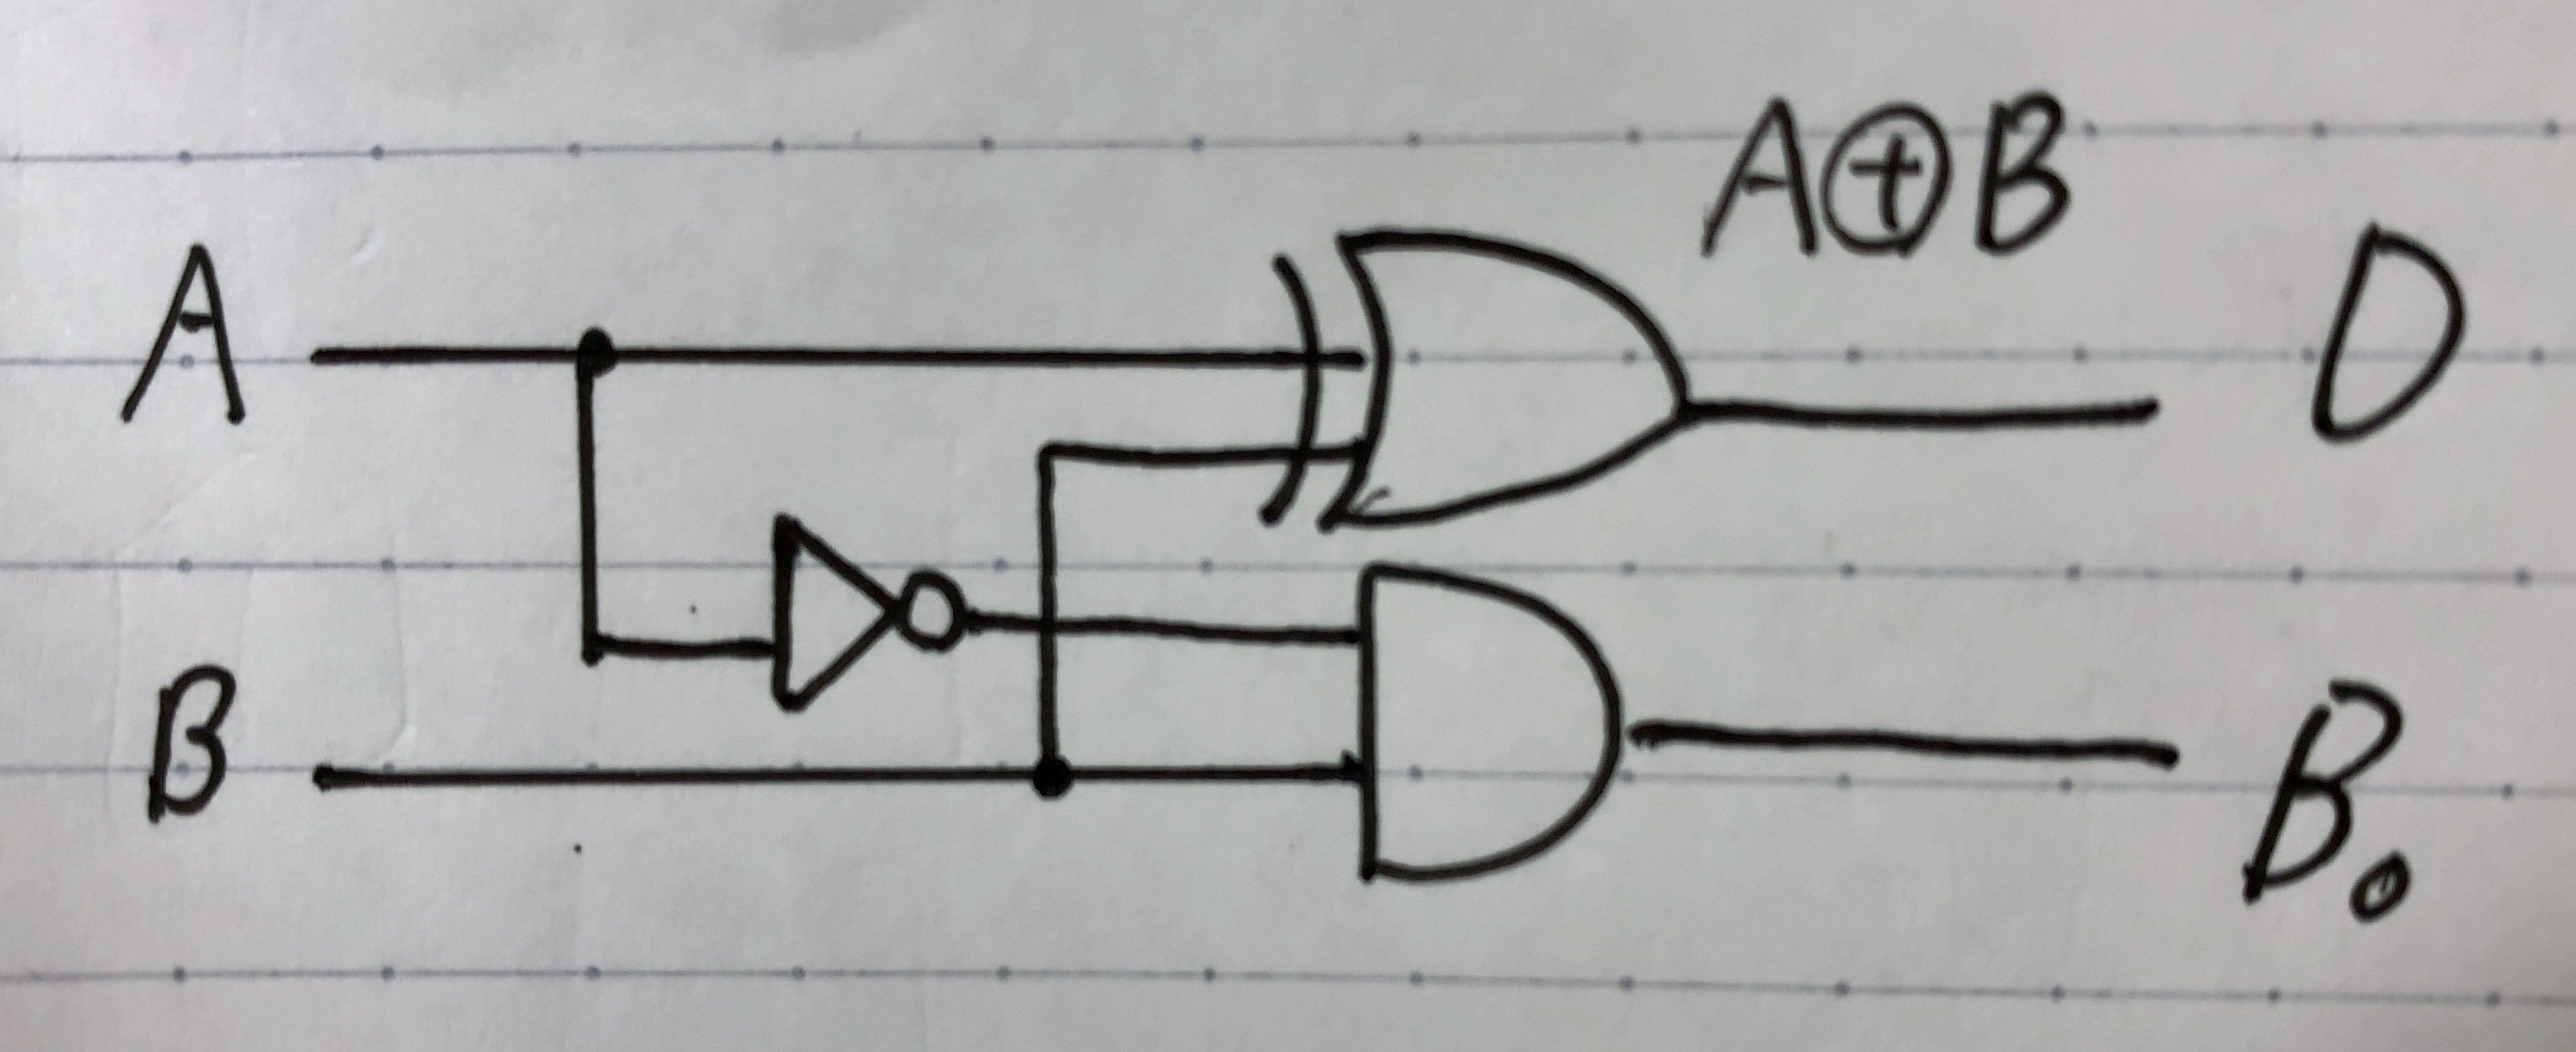
\includegraphics[bb=0 0 3616 1477,height=4cm]{report3_fig1.jpg}
              \end{center}
              \caption{半減算回路}
              \label{fig1}
          \end{figure}

          \clearpage

    \item 全減算器

          半減算器は1ビット(一桁)の減算なので、二桁以上の減算を行うには不完全で
          下位桁からの借りを考慮しないといけない。
          下位桁からの借りを$B_i$、上位桁からの借りを$B_O$として
          その桁の減算を完全にしたものを全減算器という。

          被減数$A$から減数$B$を引けない場合、
          上位桁への借り$B_O$は上位桁において下位桁からの借り$B_i$として入力され、
          $D = A - B - B_i$とすると、
          全減算器の真理値表は、表\ref{repotbl5}のようになる。
          \begin{table}[h]
              \caption{半減算器の真理値表}
              \begin{center}
                  \begin{tabular}{|ccc|cc|}
                      \hline
                      \multicolumn{3}{|c|}{入力} & \multicolumn{2}{|c|}{出力}                       \\
                      \hline
                      $A$                        & $B$                        & $B_i$ & $B_O$ & $D$ \\
                      \hline
                      0                          & 0                          & 0     & 0     & 0   \\
                      0                          & 1                          & 0     & 1     & 1   \\
                      1                          & 0                          & 0     & 0     & 1   \\
                      1                          & 1                          & 0     & 0     & 0   \\
                      0                          & 0                          & 1     & 1     & 1   \\
                      0                          & 1                          & 1     & 1     & 0   \\
                      1                          & 0                          & 1     & 0     & 0   \\
                      1                          & 1                          & 1     & 1     & 1   \\
                      \hline
                  \end{tabular}
              \end{center}
              \label{repotbl5}
          \end{table}

          真理値表より、全減算回路は図\ref{fig2}のようになる。
          点線で囲っているのは半減算回路である。
          \begin{figure}[h]
              \begin{center}
                  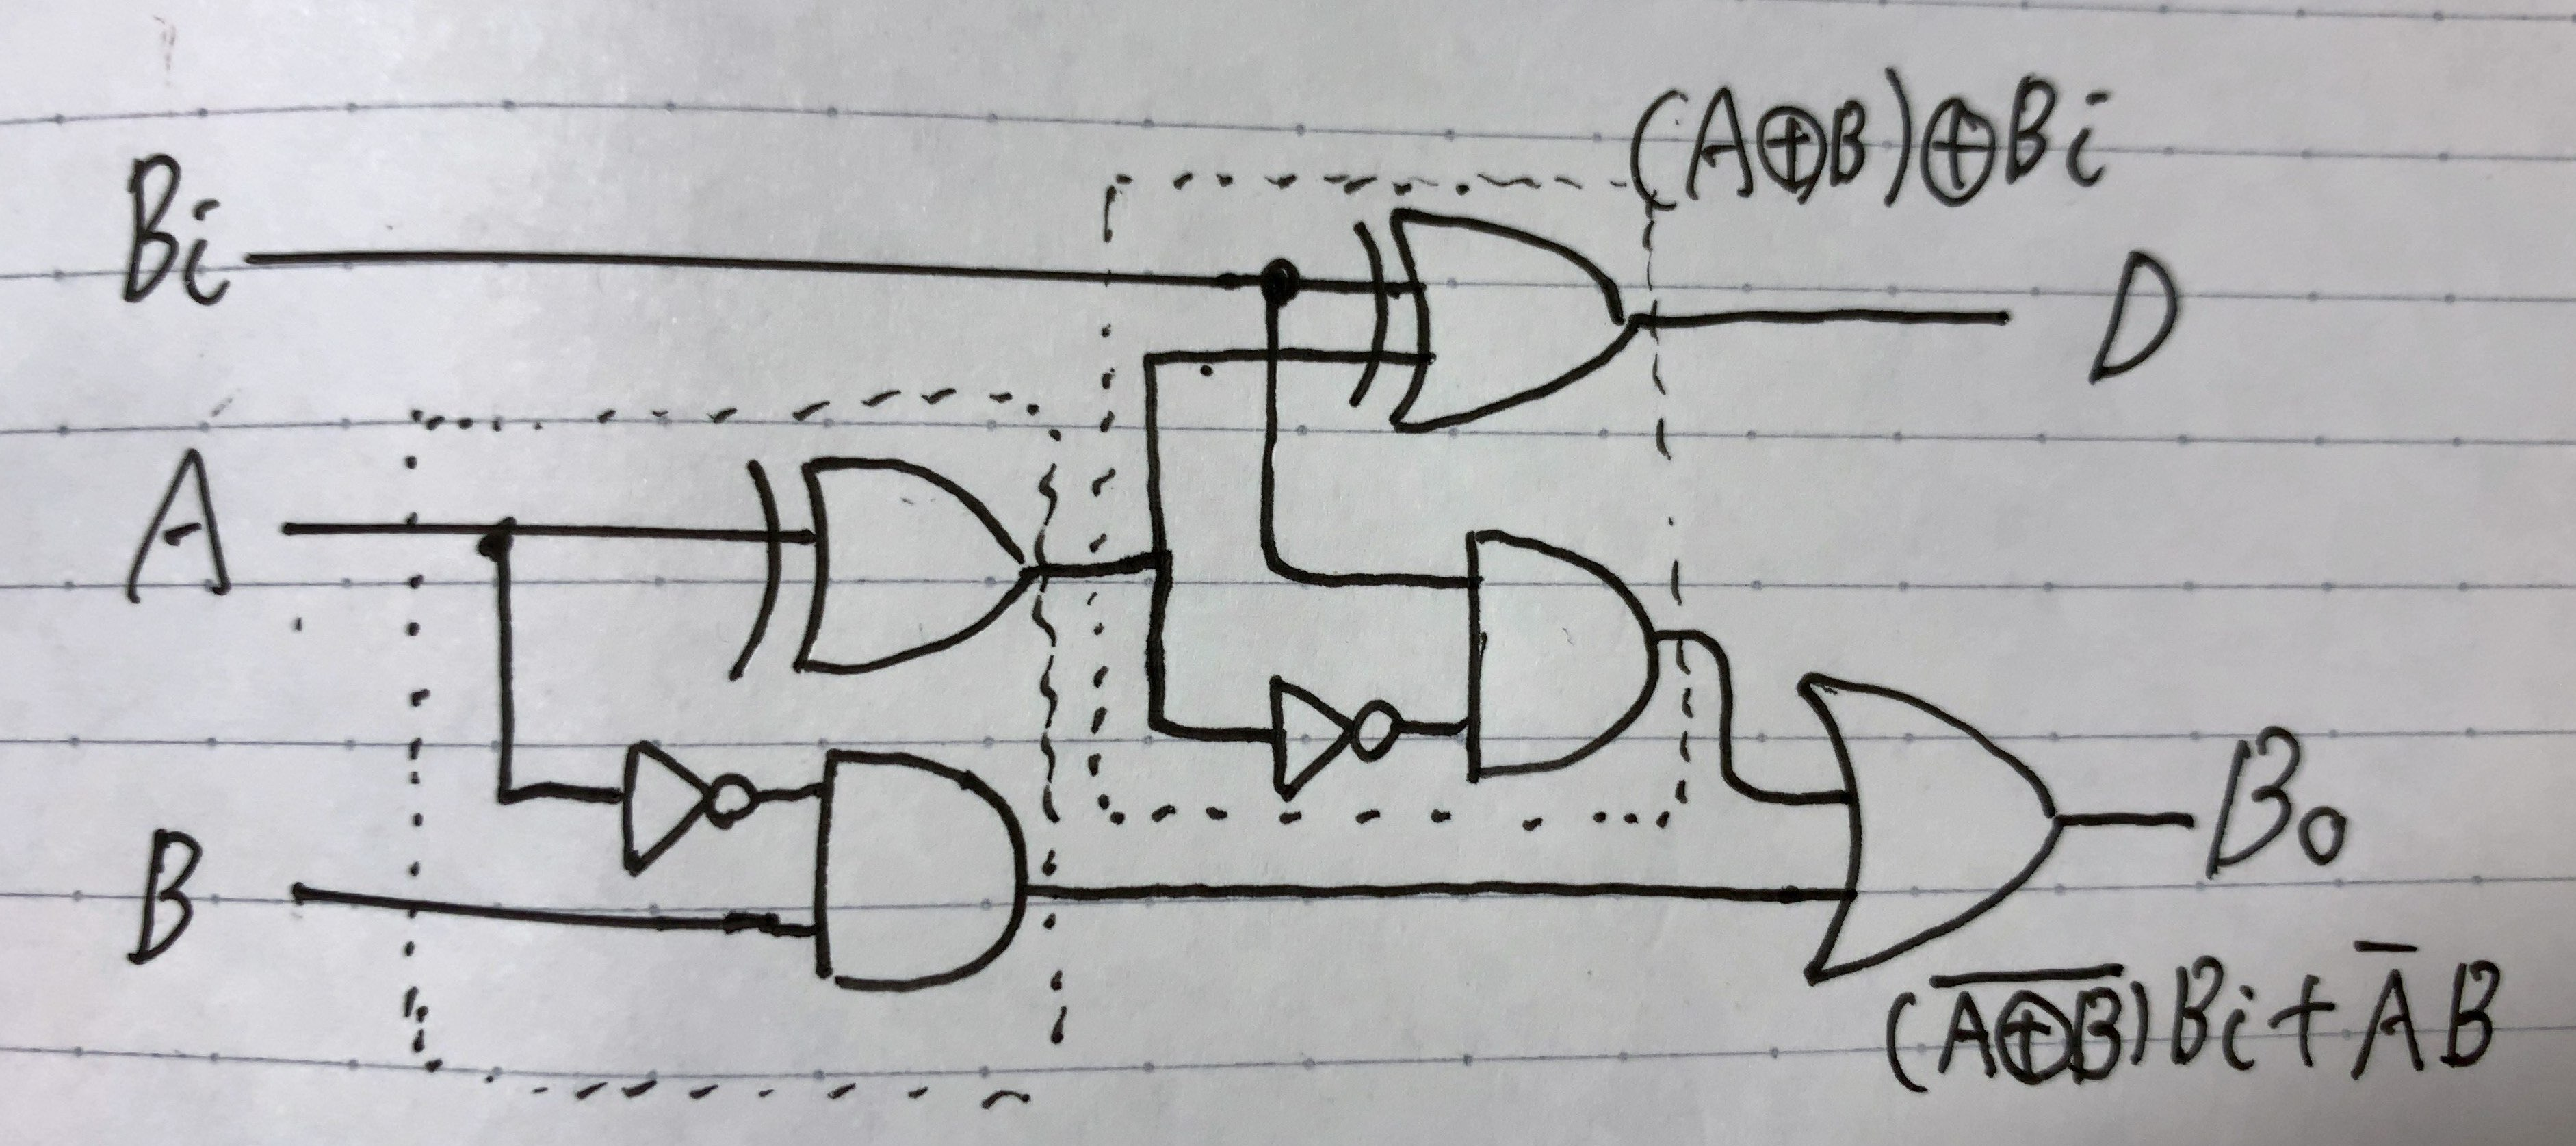
\includegraphics[bb=0 0 4032 3024,height=8cm]{report3_fig2.jpg}
              \end{center}
              \caption{全減算回路}
              \label{fig2}
          \end{figure}
\end{itemize}

\clearpage
\subsection{レポート課題4}
\begin{shadebox}
    10進カウンタの動作をタイムチャートで示せ。
    その上で、同期式・非同期式の10進カウンタ回路をそれぞれ示し、
    動作原理を説明せよ。
\end{shadebox}
\subsubsection*{非同期式10進数カウンタ回路}
非同期式10進数カウンタ回路のタイムチャートと回路は、
それぞれ図\ref{fig5}、図\ref{fig6}に示した。

右端のNANDゲートの出力は通常は1であるが、
カウンタの値が0、1、2、と進み10($Q_2=0$、$Q_3=0$)になったとき、
NANDゲートの出力が0となる。
この出力は全てのフリップフロップのクリア端子につながっていて、
この回路ではクリア端子は負論理であるから、
0になったとき、クリアが実行される。
すなわち、カウンタの値は0になる。

タイムチャートを見れば分かるように、
短い期間でカウンタの値が10となっている。
このヒゲ状のノイズが問題にならないときはこのような簡単な方法で
2のN乗以外のカウンタを作ることができる。
\begin{figure}[h]
    \begin{center}
        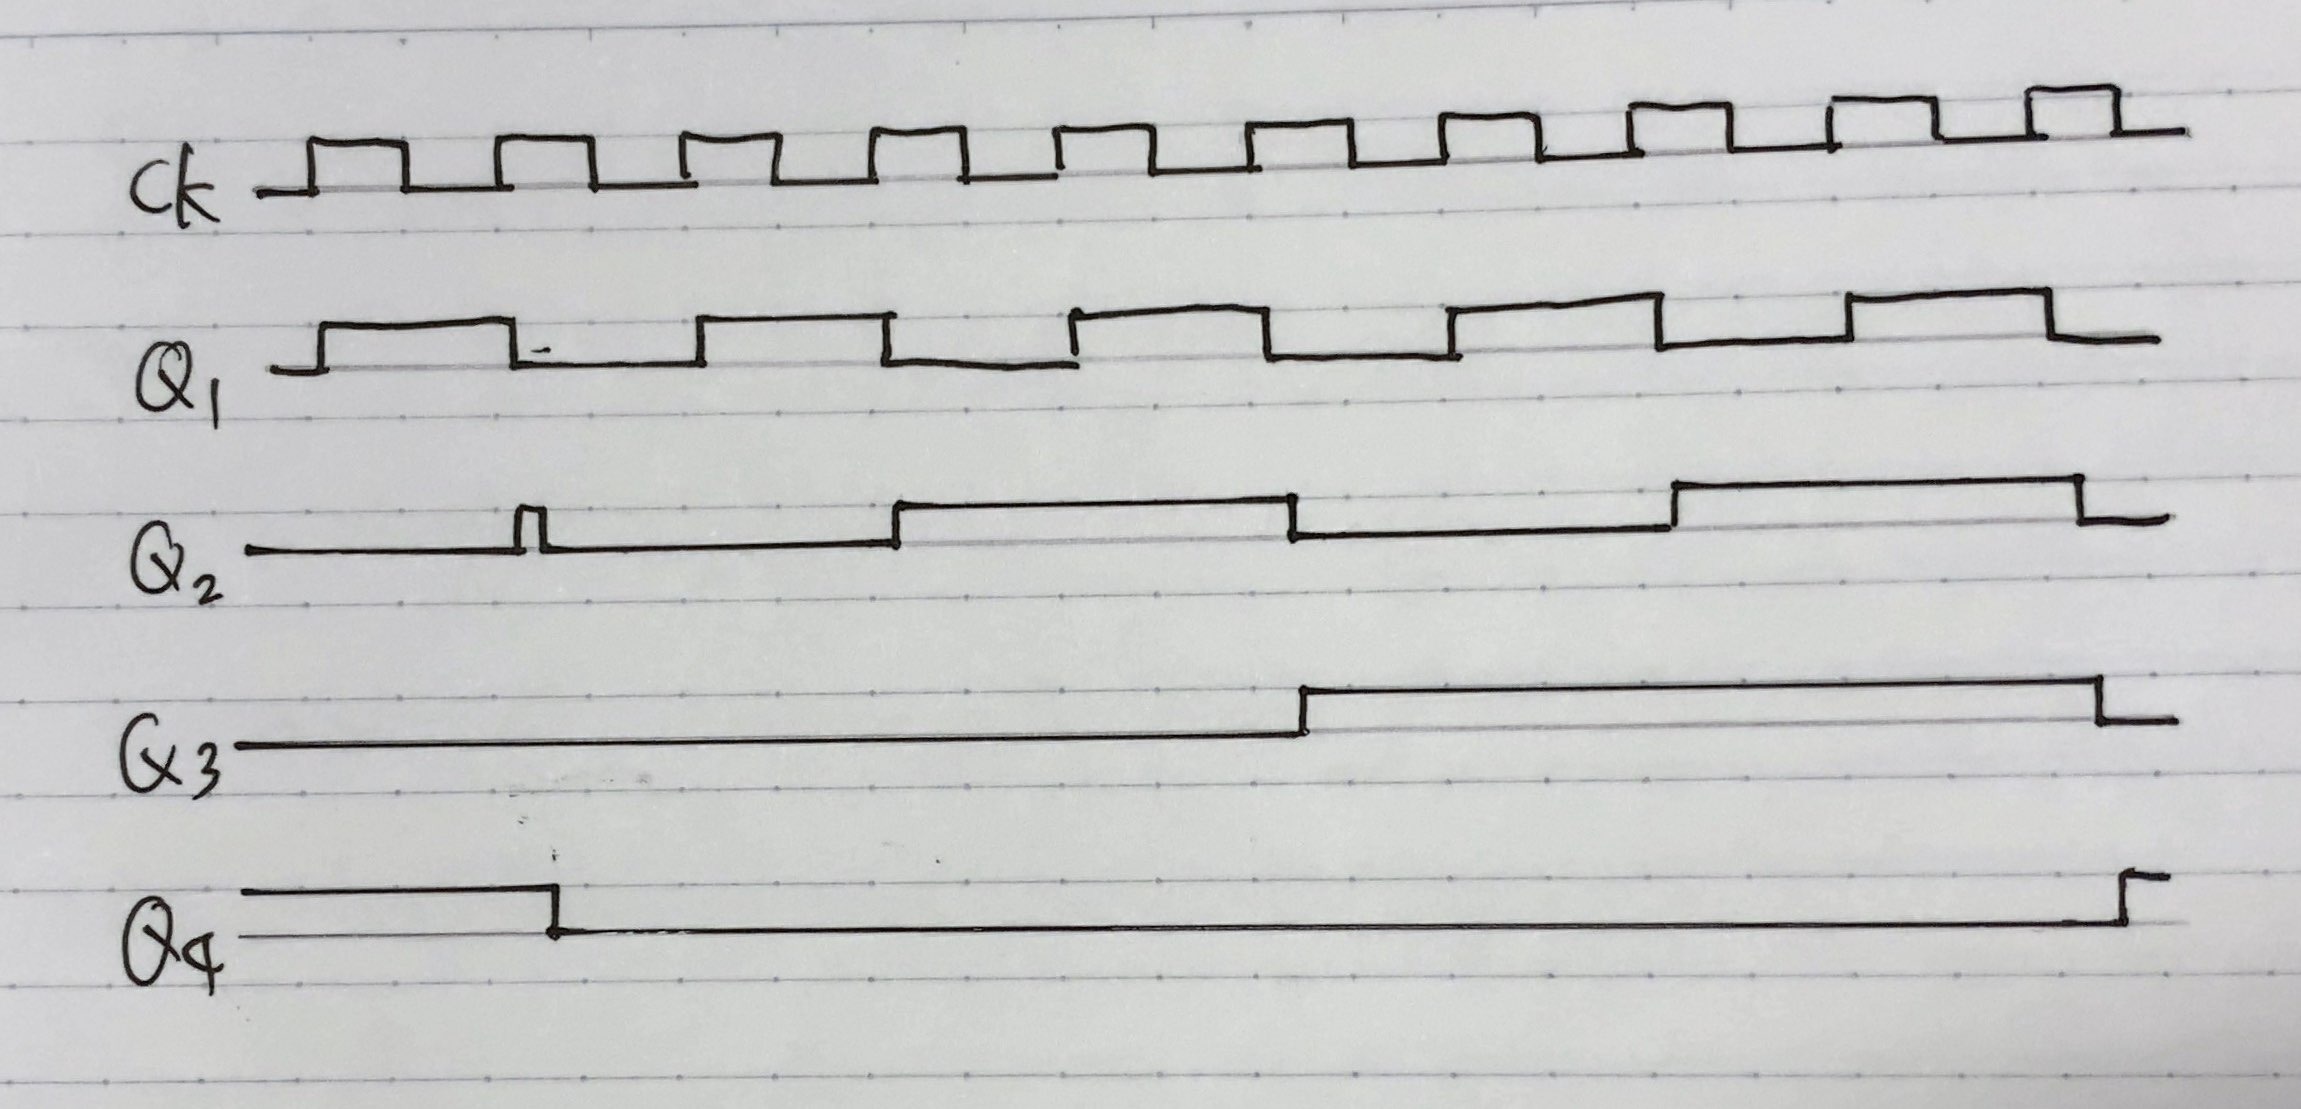
\includegraphics[bb=0 0 2301 1109,height=6cm]{report3_fig5.jpg}
    \end{center}
    \caption{非同期式10進数カウンタのタイムチャート}
    \label{fig5}
\end{figure}
\begin{figure}[h]
    \begin{center}
        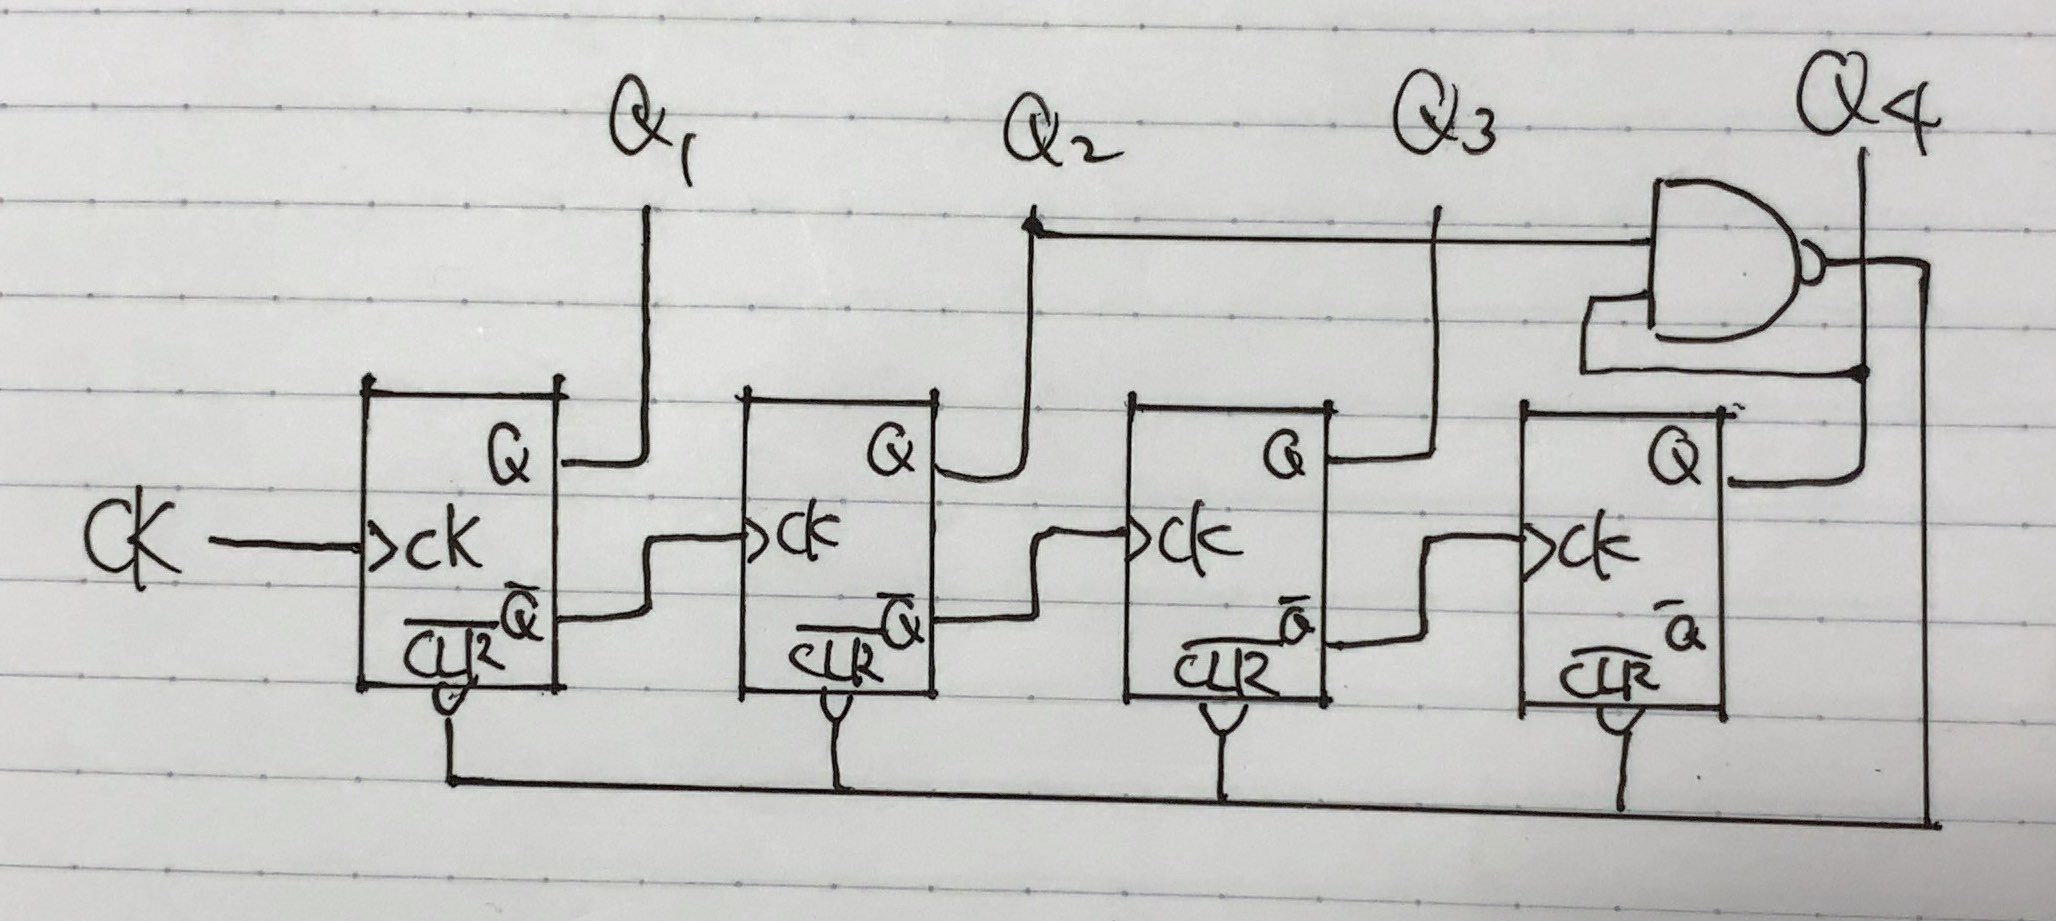
\includegraphics[bb=0 0 2056 921,height=6cm]{report3_fig6.jpg}
    \end{center}
    \caption{非同期式10進数カウンタ回路}
    \label{fig6}
\end{figure}

\clearpage
\subsubsection*{同期式10進数カウンタ回路}
同期式10進数カウンタ回路のタイムチャートと回路は、
それぞれ図\ref{fig3}、図\ref{fig4}に示した。

同期式カウンタとは、
カウンタを構成する全てのフリップフロップが同じクロックで動作するものである。
非同期式10進数カウンタと違い、
ヒゲ状のノイズが生まれないようにできるが、
非同期式10進数カウンタ回路より複雑である。

\begin{figure}[h]
    \begin{center}
        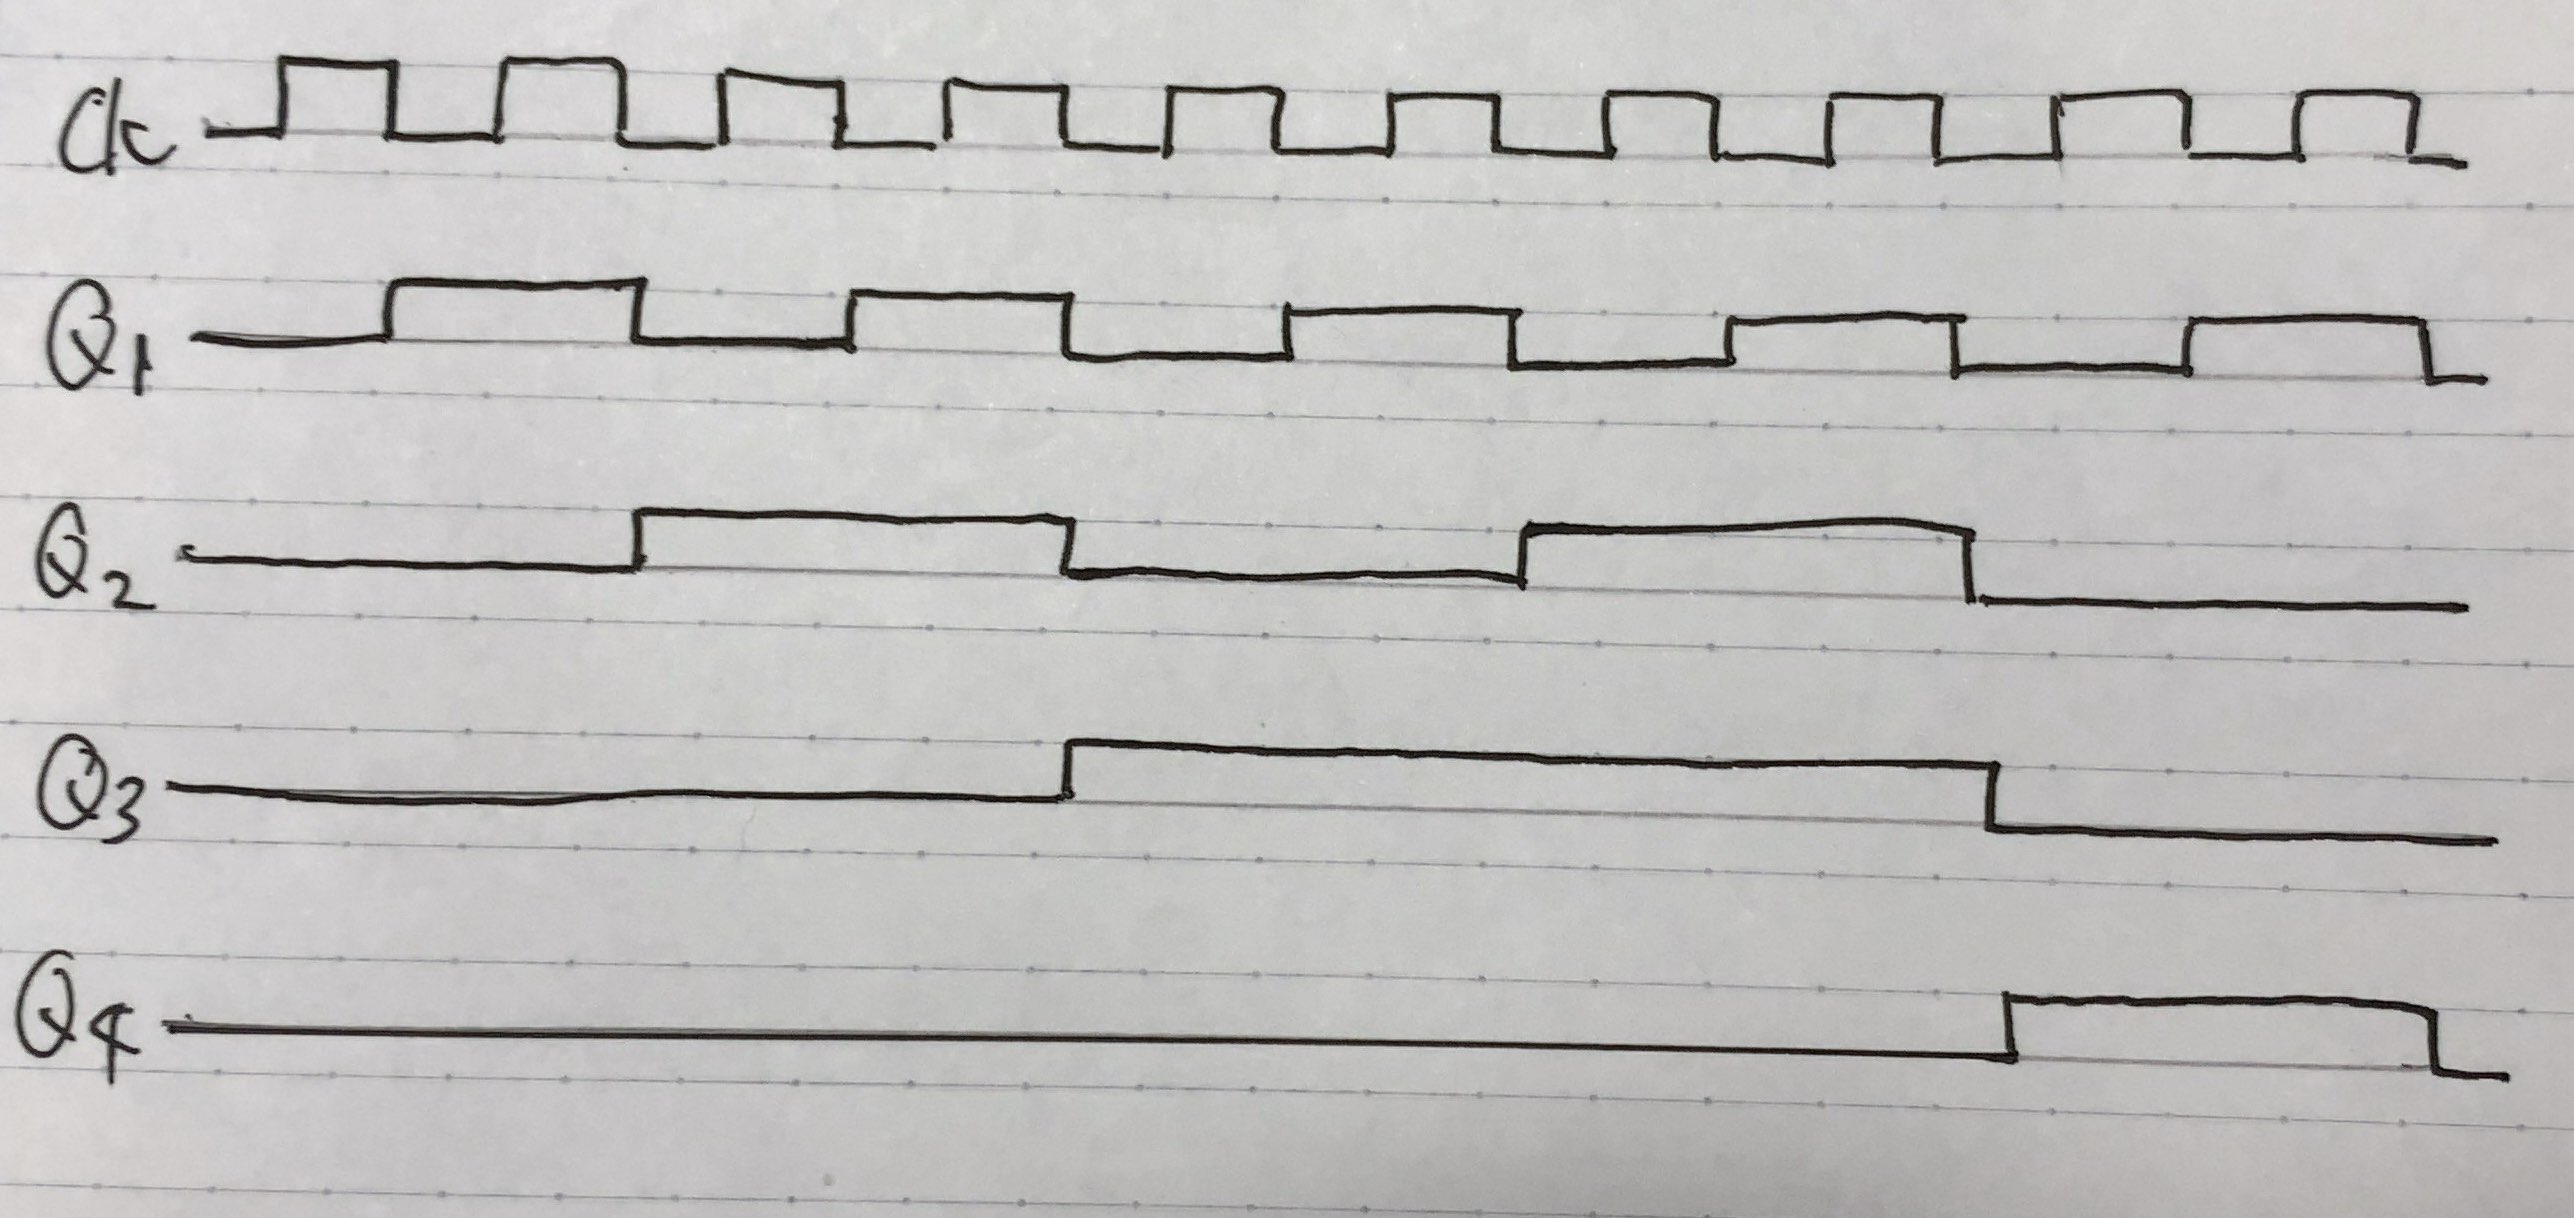
\includegraphics[bb=0 0 2574 1218,height=7cm]{report3_fig3.jpg}
    \end{center}
    \caption{同期式10進数カウンタのタイムチャート}
    \label{fig3}
\end{figure}
\begin{figure}[h]
    \begin{center}
        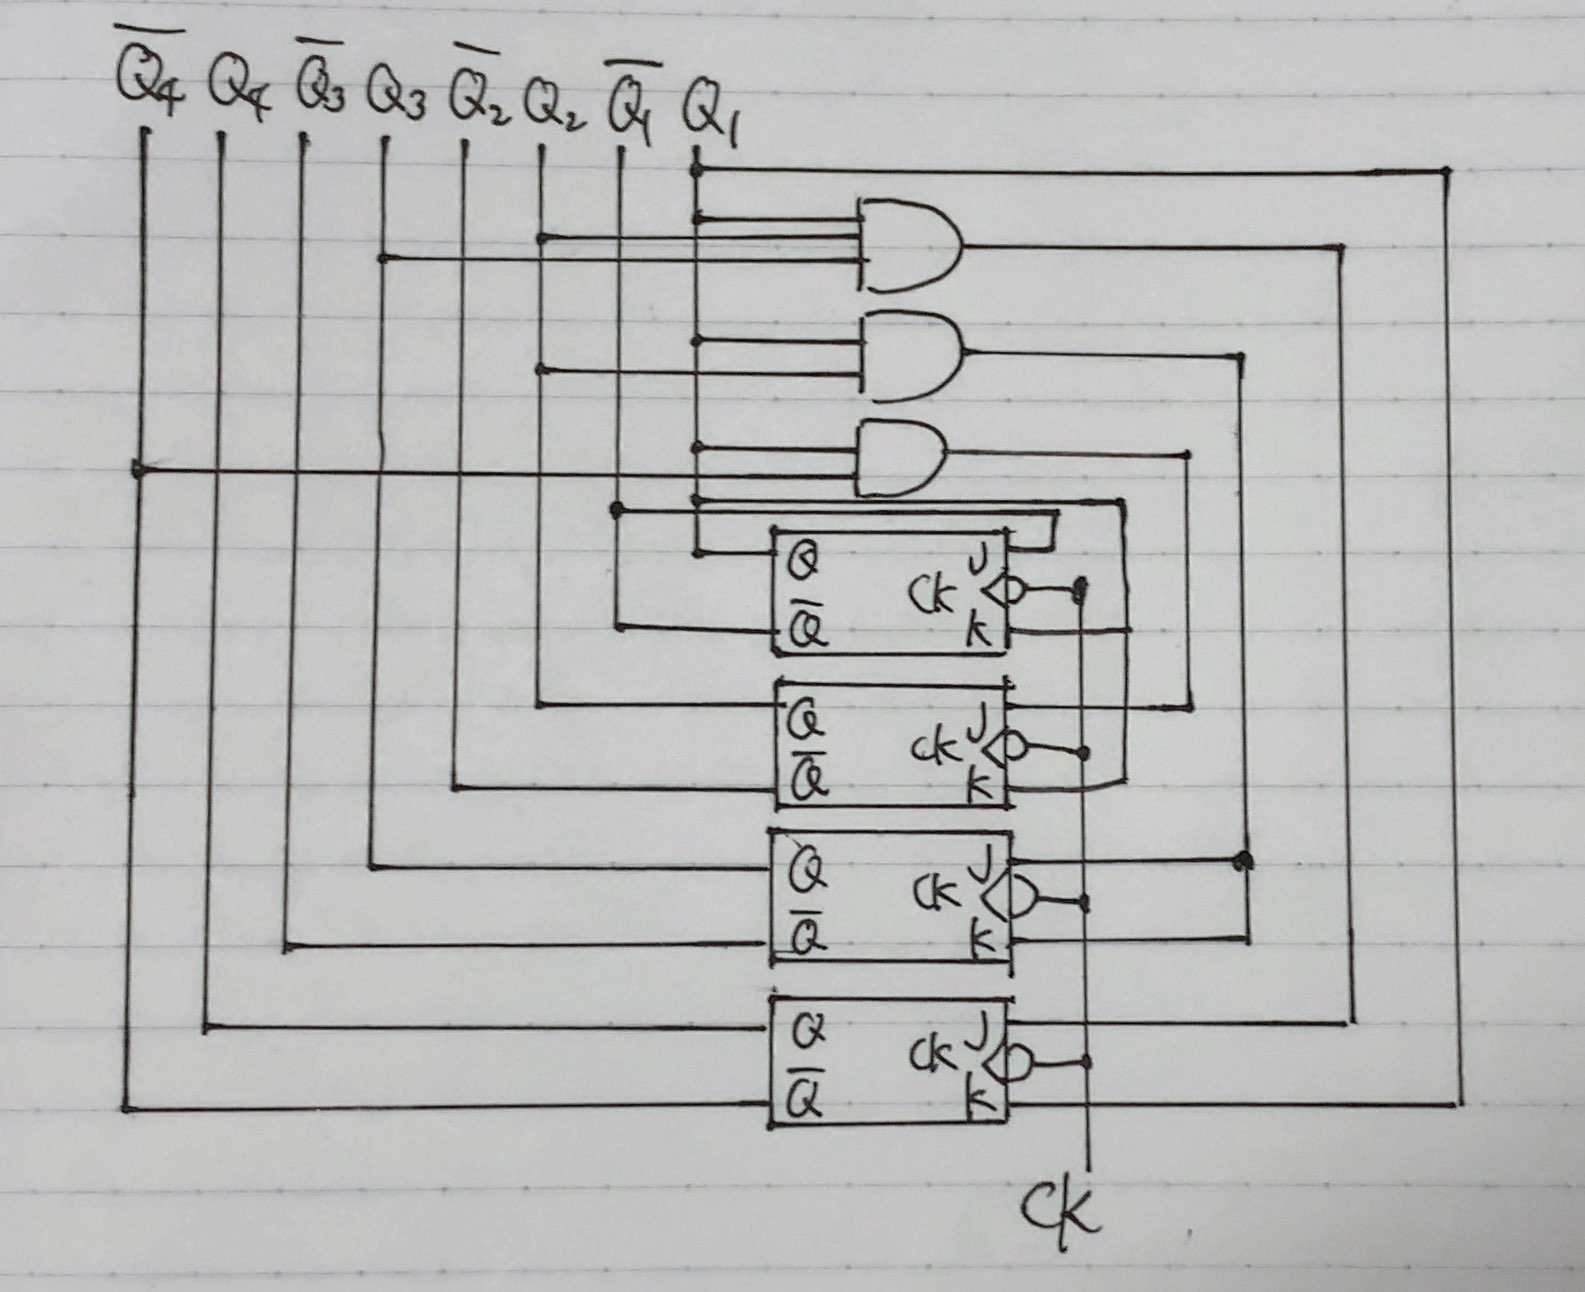
\includegraphics[bb=0 0 1585 1292,height=8cm]{report3_fig4.jpg}
    \end{center}
    \caption{同期式10進数カウンタ回路}
    \label{fig4}
\end{figure}

\clearpage
\section{結論}
本実験では、ディジタル回路の設計・解析に必要な基本となるゲート素子
の基礎的動作原理を理解することができた。
また、応用であるカウンタ回路などでは、
トリガが重要であることが分かった。

% 参考文献
\begin{thebibliography}{99}
    \label{sannkoubunnkenn_chapter}
    \bibitem[1]{rikadai}東京理科大学工学部情報工学科「情報工学実験1 2020年度」
    (2020/4/6)

    \bibitem[2]{circuit}大類重範「ディジタル電子回路」
    日本理工出版会(2017/5/15)

    \bibitem[3]{douki_counter}同期式カウンターJKフリップフロップ使用(1)

    \url{http://home.a00.itscom.net/hatada/dc2/chap13/syn_counter_jkff1.html}

    最終閲覧日:2020/6/17

    \bibitem[4]{hidouki_counter}非同期式カウンタ

    \url{http://home.a00.itscom.net/hatada/dc2/chap12/counter.html}

    最終閲覧日:2020/6/17
\end{thebibliography}

\clearpage
\appendix
%%%%%%%%%%%%%%%%%%%%%%%%%%%%%%%%%%%%%%%%%%%%%%%%%%%%%%%
\end{document}
